\section{Perceptrons}
\smallskip \hrule height 2pt \smallskip

\begin{itemize}
	\item Error driven, not probabilistic. \hfill \\
		\begin{itemize}
			\item Mistake driven rather than model drive. \hfill \\
			\item Parameters from reactions to mistakes  % end of slide set 7
		\end{itemize}
	\item Parameters are from a discriminative interpretation % end of slide set 7
	\item To train, you go through the data until the held-out accuracy maxes out. % end of slide set 7
	\item Note you can scale your $w$ (weight) vector(s) by any constant because all you care about is sign($w \cdot x$).
		This rescales your gamma by that constant too! \hfill \\
\end{itemize}

\subsection{Properties of Perceptron}
\underline{Separability}: some parameters get the training set perfectly correct. \hfill \\
\underline{Convergence}: if the training is separable, the perceptron will eventually converge. \hfill \\
\underline{Mistake Bound}: the maximum number of mistakes (for the binary case) is related to the 
margin or degree of separability: $mistakes \leq \frac{R^2}{\gamma^2}$. \hfill \\

\subsection{Problems with the Perceptron}
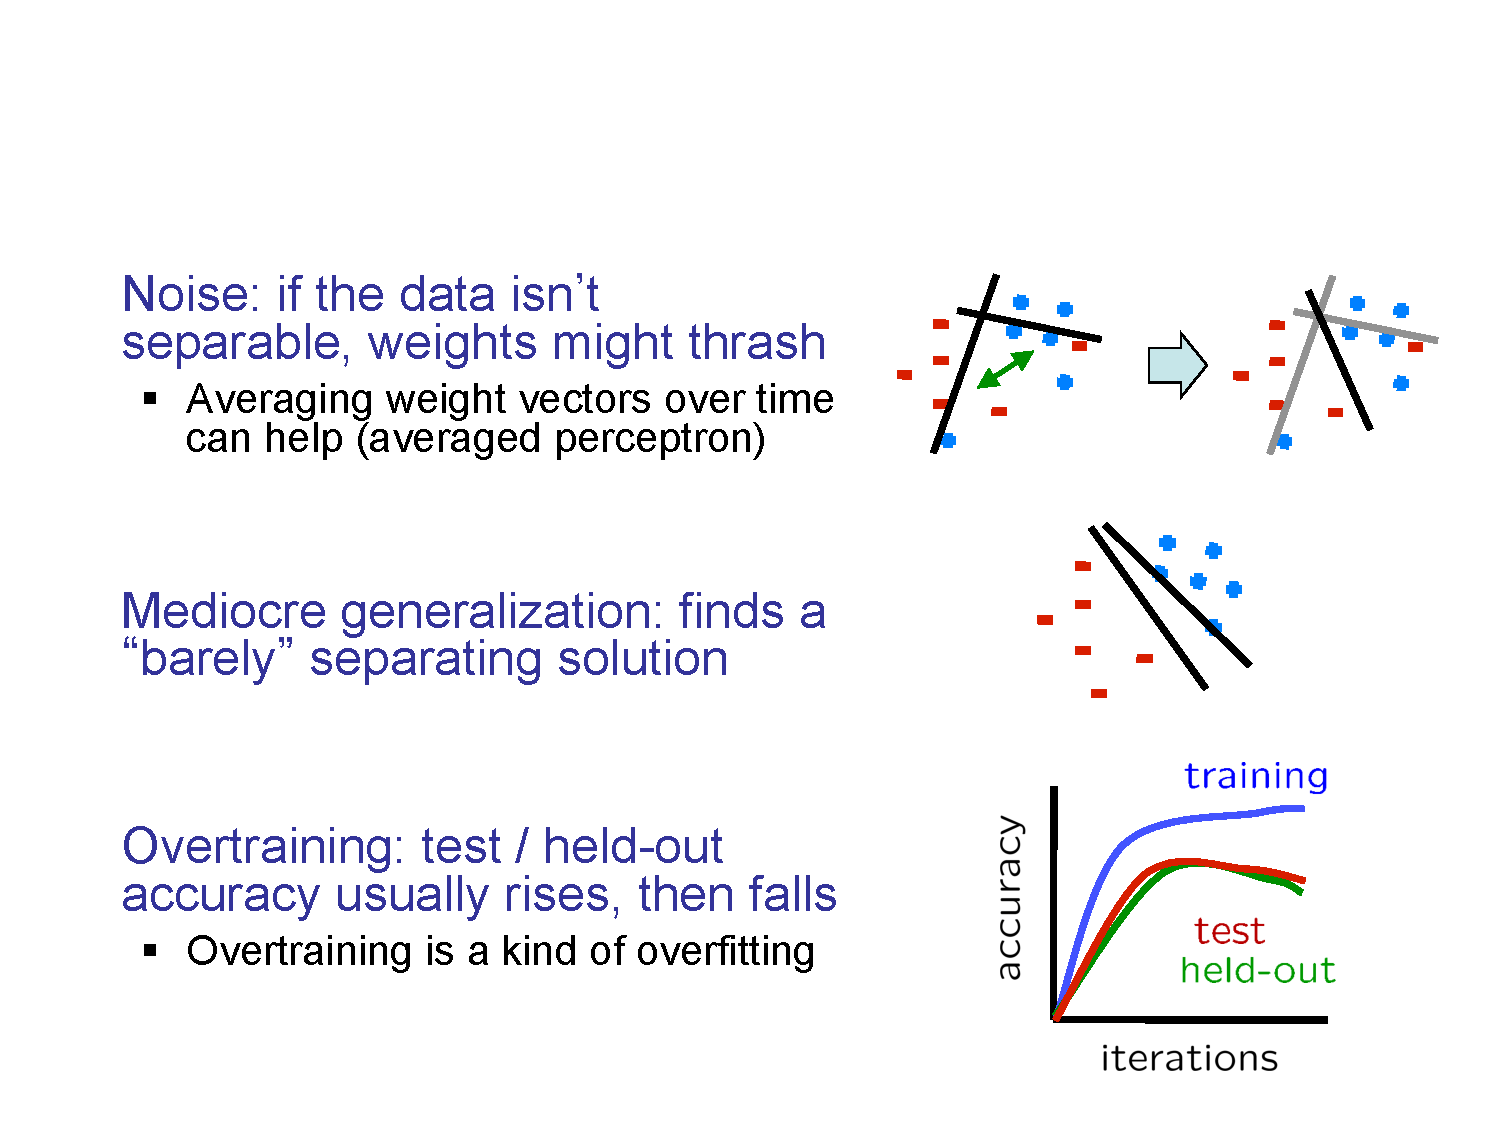
\includegraphics[width=2.8in]{figures/perceptron_problems.pdf}

 \subsection{Linear Classifiers}
 Inputs are feature values.  \hfill \\
 Each feature has a weight.  \hfill \\
 Sum is the activation.  activation$_w(x) = \sum_i w_i x_i = w \cdot x$  \hfill \\
 If the activation is positive, chose output class 1.  \hfill \\
 If the activation is negative, chose output class 2.  \hfill \\
 
 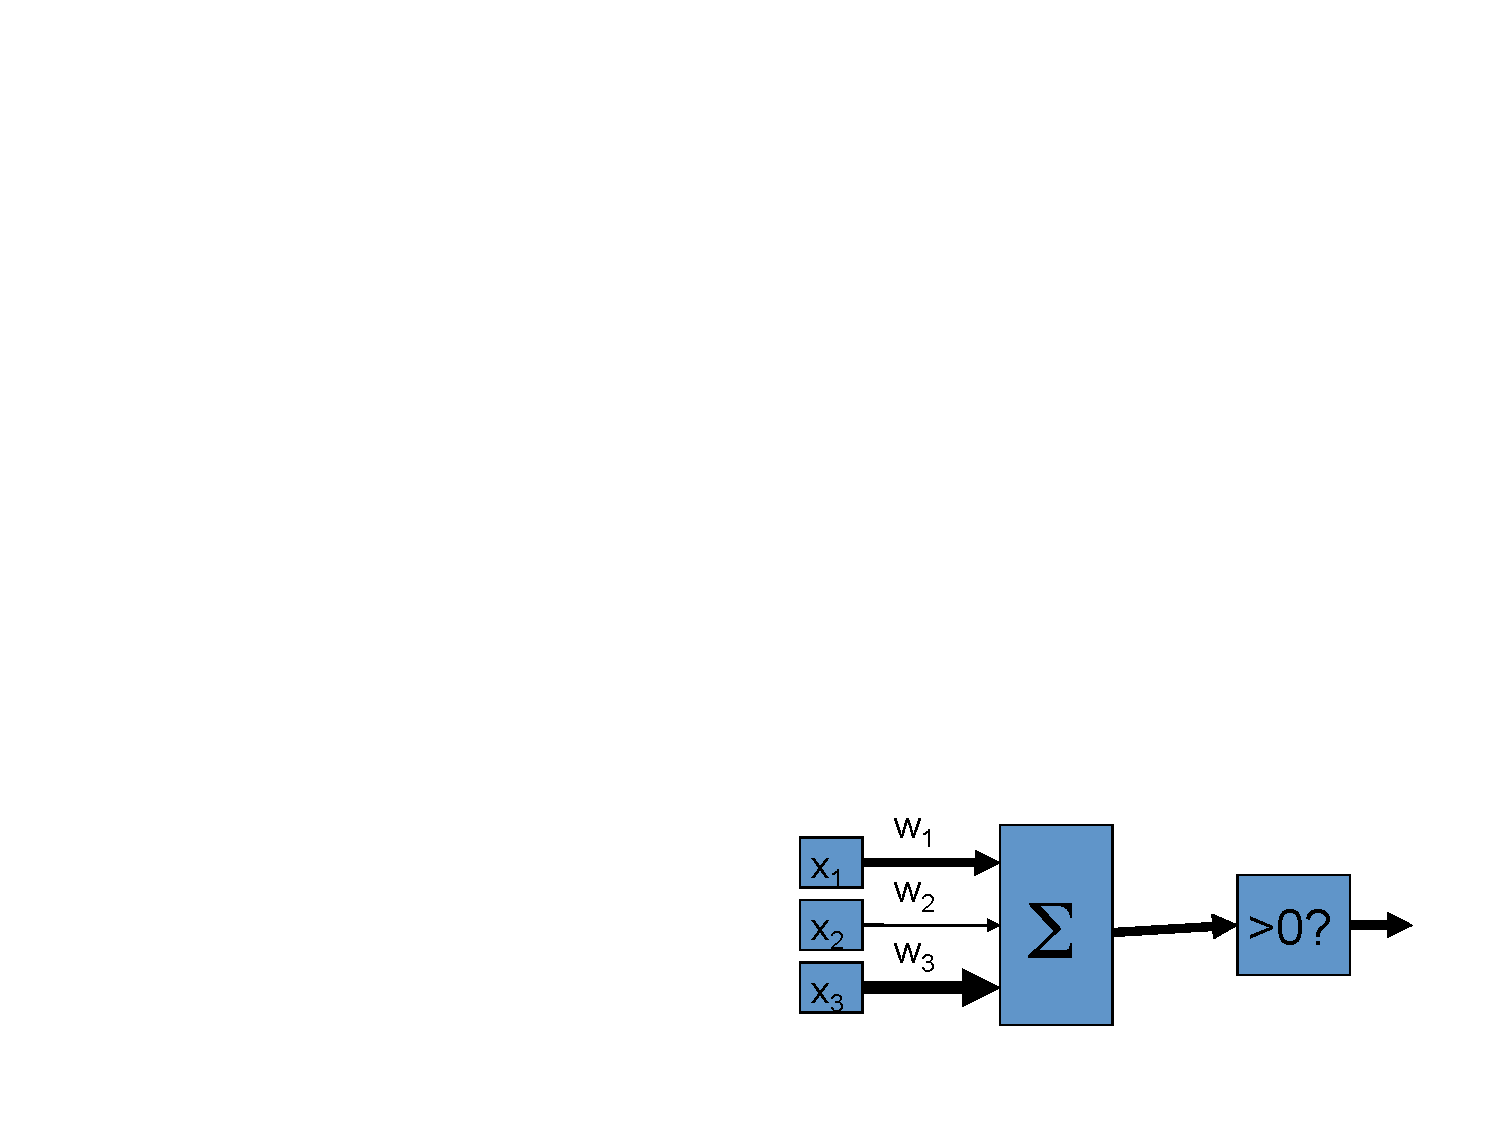
\includegraphics[width=1.5in]{figures/linear_classifier_cartoon.pdf}  \hfill \\
 
 For a binary decision rule:   \hfill \\
 In the space of feature vectors: 
 \begin{itemize}
 	\item examples are points
	\item any weight vector is a hyperplane
	\item one side corresponds to y = +1
	\item the other side corresponds to y = -1
	\item ??? The $w \cdot x = 0$ is the solution to the line.
 \end{itemize}
 
 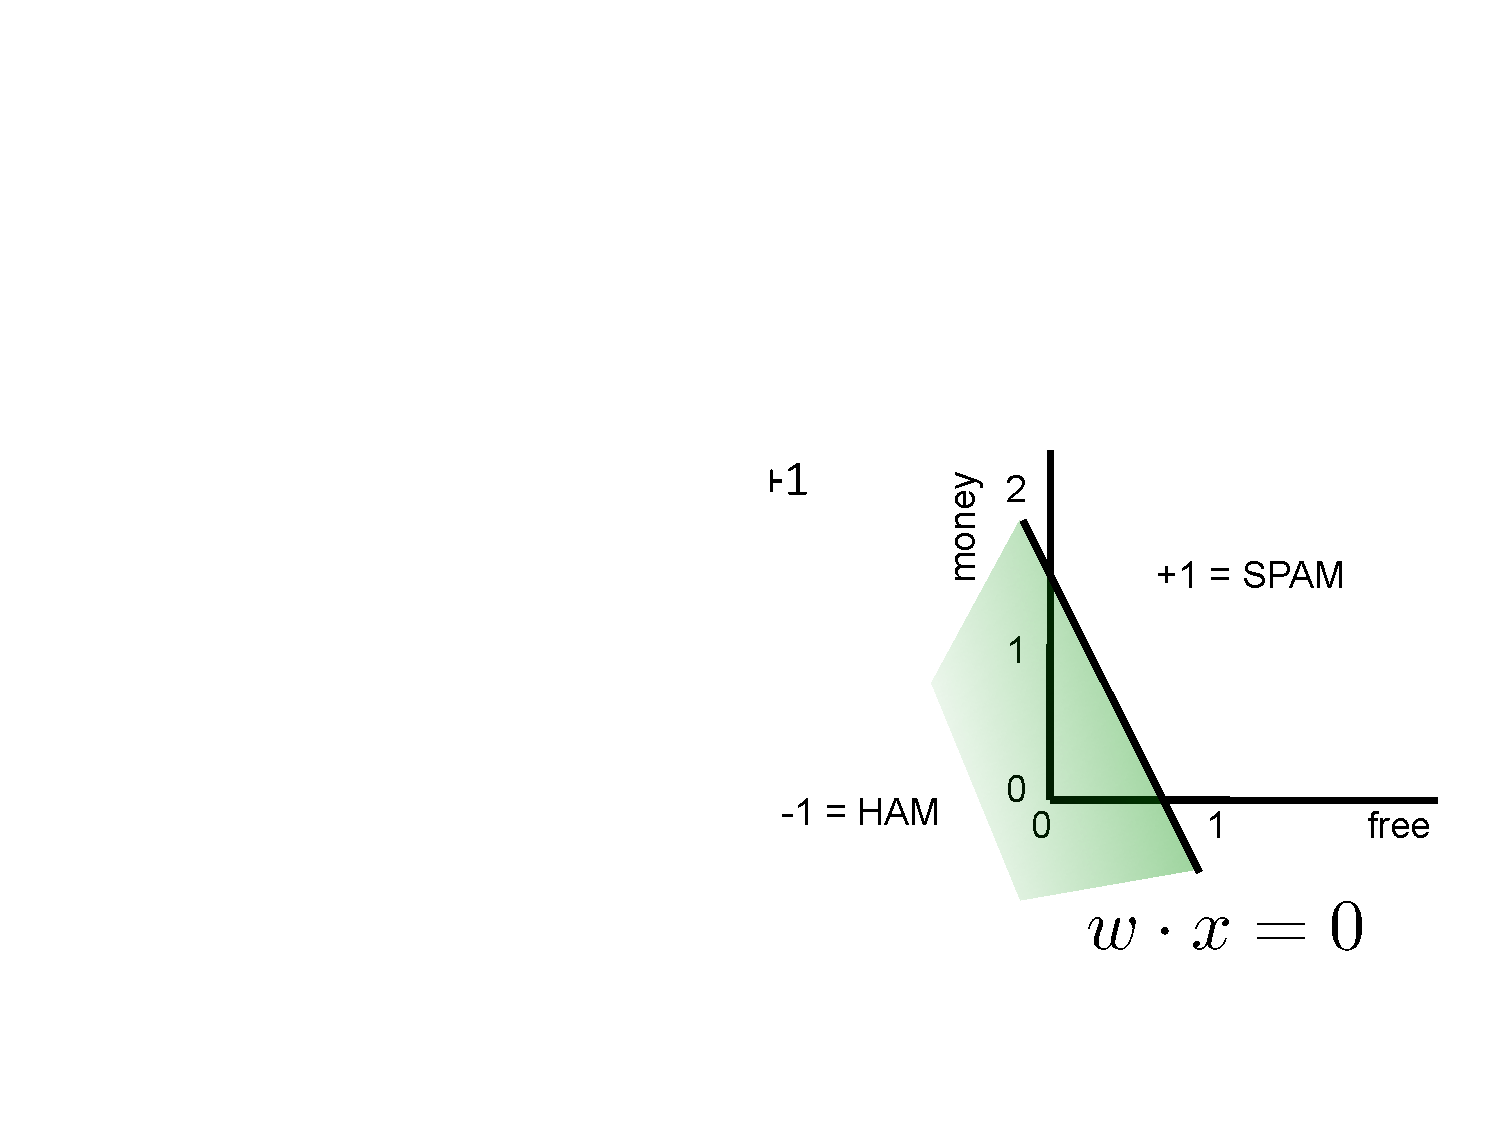
\includegraphics[width=1.5in]{figures/binary_decision_rule.pdf}
 
 \subsubsection{Binary Perceptron Algorithm}
 \begin{itemize}
 	\item start with zero weights: $w=0$
	\item for $ t = 1 \dots T$ (T passes over the data):
		\begin{itemize}
			\item for $i = 1 \dots n$ (each training example)
			\begin{itemize}
				\item  Classify with current weights: \hfill \\
					$ y = sign(w \cdot x^i)$ \hfill \\
					(sign($z$)  is $+1$ if $z > 0$, else -1) \hfill \\
				\item if correct (i.e. $y = y^i$), don't change weights.
				\item if it was wrong, update with $w = w + y^i x^i$
			\end{itemize}
		\end{itemize}
 \end{itemize}
 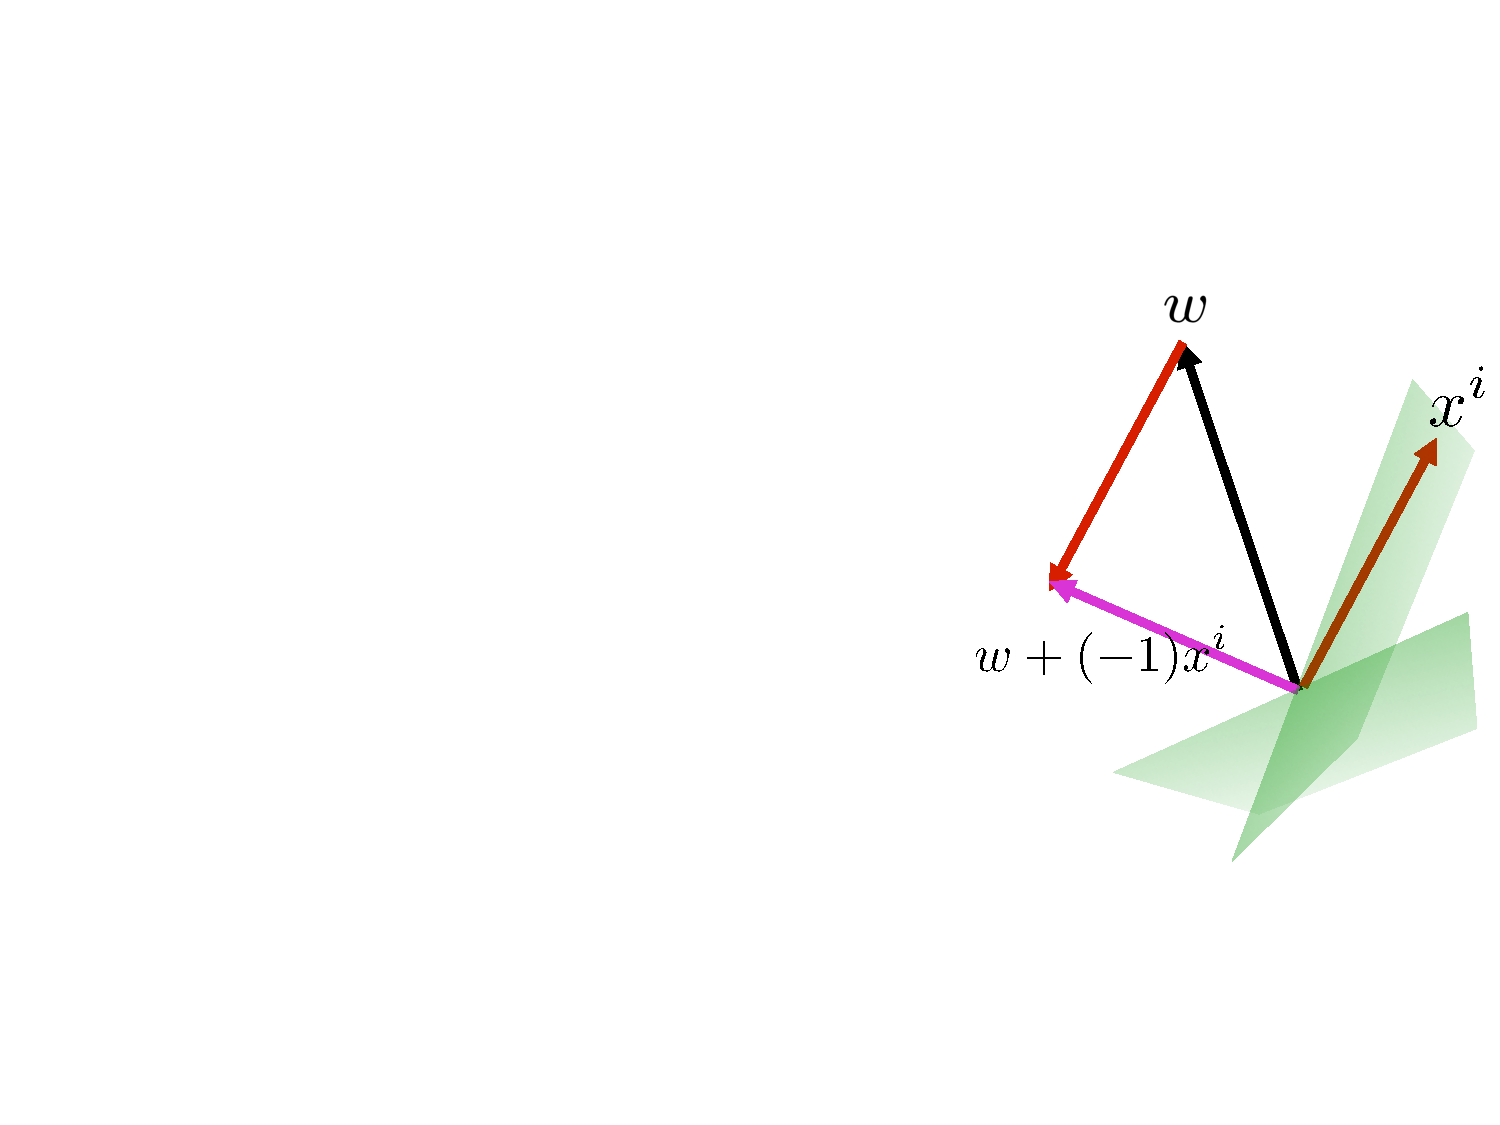
\includegraphics[width=1.0in]{figures/binary_perceptron_rule.pdf}
  
 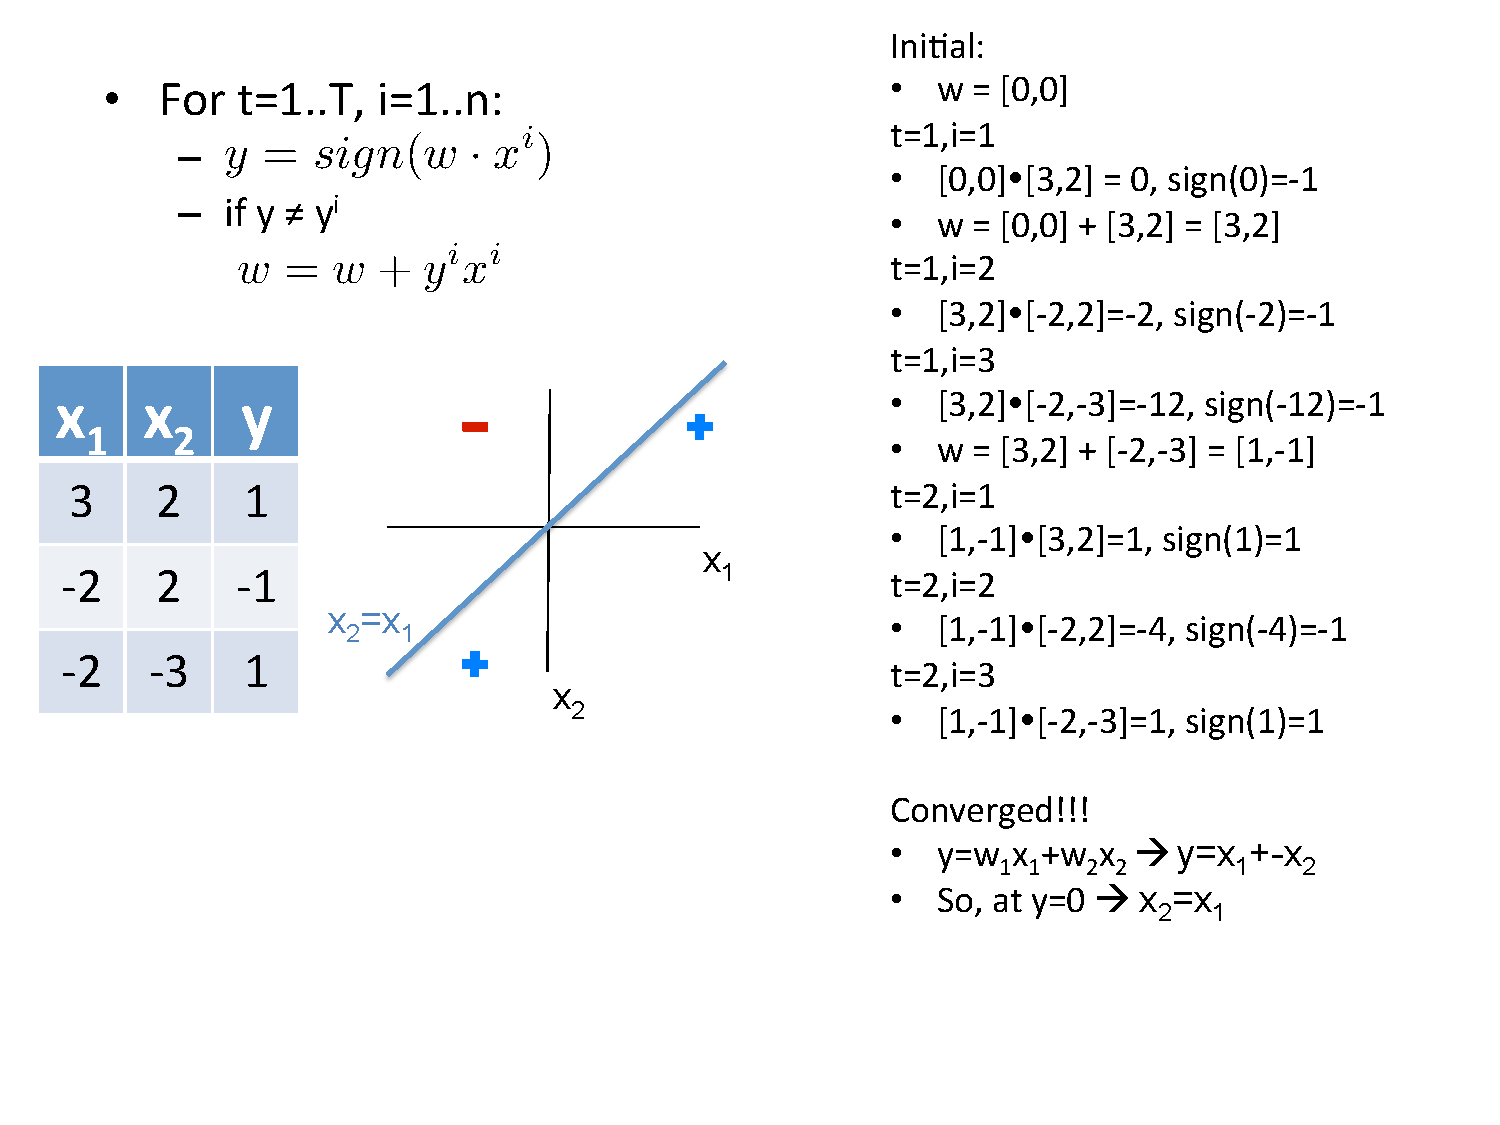
\includegraphics[width=3.2in]{figures/perceptron_chugging_example.pdf}
 
 \underline{$w \cdot x$ and the boundary between positive and negative answers} \hfill \\
If a point has w * x = 1000, a small change in x might change w * x' to 999, or 1001, but it surely won't make w * x a negative value. On the other hand, if w * x = 0.0001, even tiny changes to x might make w * x' negative. And by extension, cases where w * x = 0 where even the tiniest change might make w * x' change sign. So the values where w * x = 0 are those that are on the boundary between positive and negative examples.[1]

So \textbf{the equation w * x = 0 defines the boundary between the positive and negative region}. Now let's unpack that statement. w is a fixed vector, while x is a variable point. So think of w = [w1, w2] as constants, and x = [x1, x2] as variables. The equation w * x = 0 is just another way of writing the equation w1 x1 + w2 x2 = 0. But this is a linear equation in two variables, so it defines a line. You can algebraically solve the equation for x2, and that gives you the "standard form" of the equation of a line, which you can then draw.

[1] The boundary of a region is defined as the set of points where even points very close by can be outside that region.

 
 \subsection{Multiclass Decision Rule}
 If we have more than two classes: 
 \begin{itemize}
 	\item we have a weight vector for \textbf{each} class: $w_y$
	\item we calculate an activation for each class: \hfill \\
		activation$_w(x,y) = w_x \cdot x$
	\item the highest activation wins:  \hfill \\
		$y^* = \argmax_y(activation_w(x,y))$ \hfill \\
		"win the vote" 
 \end{itemize}
 
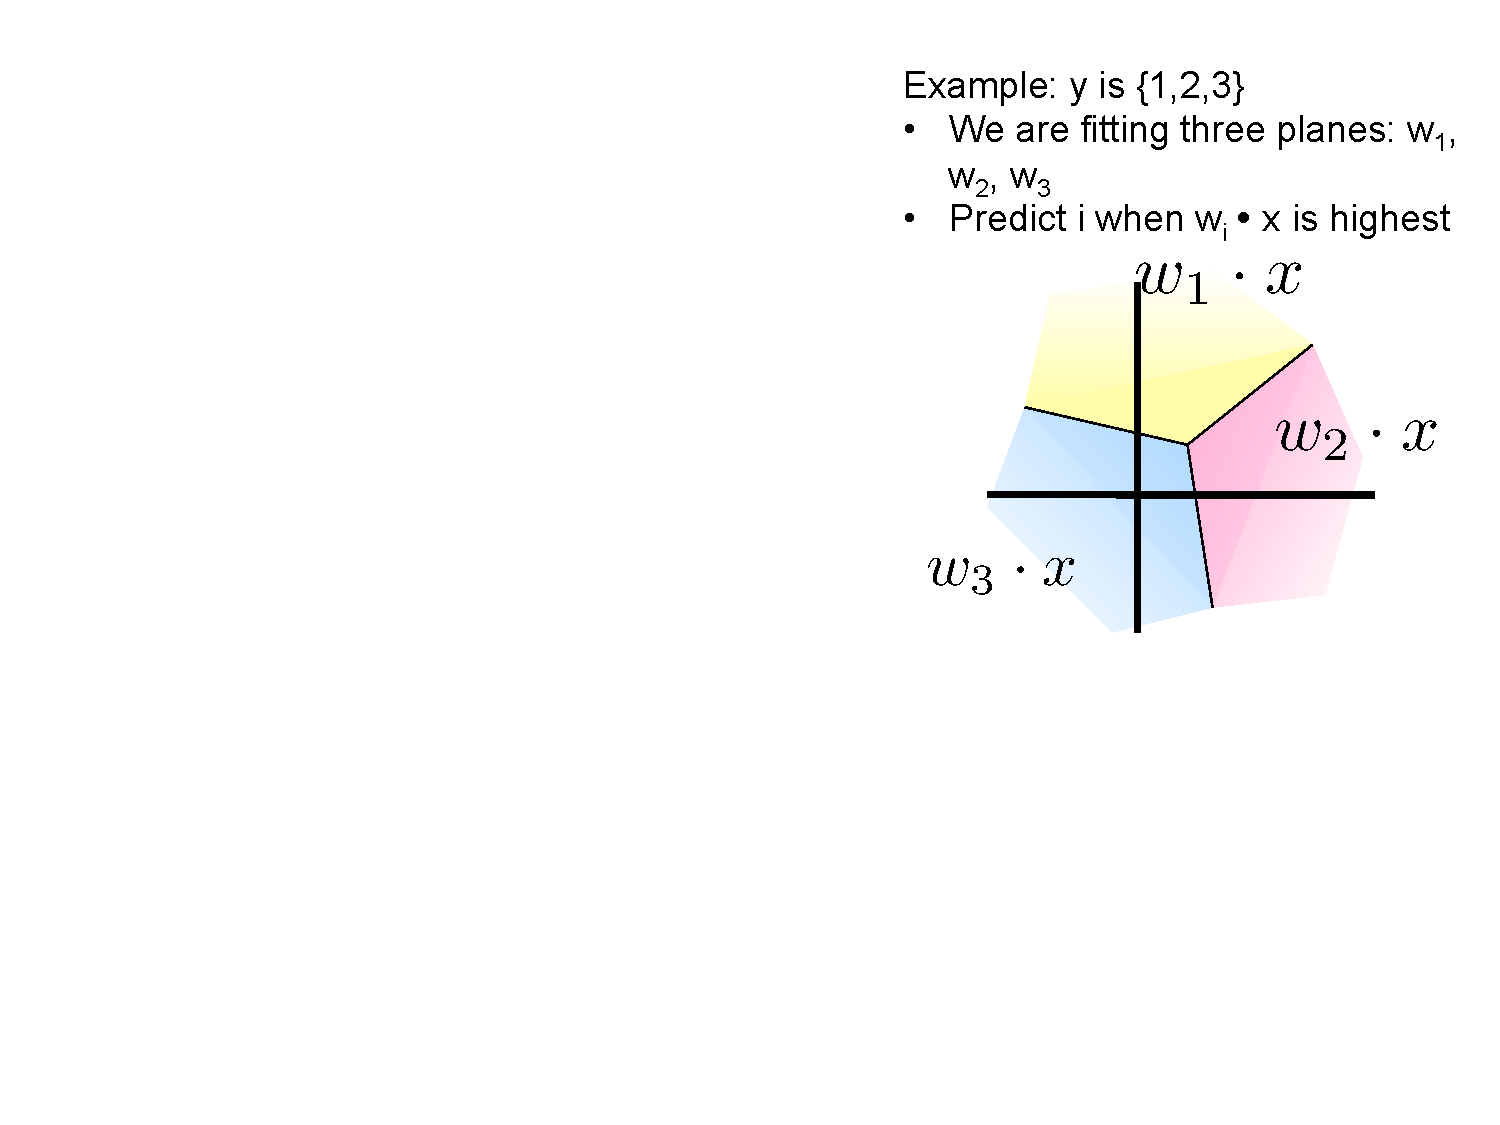
\includegraphics[width=1.5in]{figures/multiclass_decision_rule_planes.pdf}
 
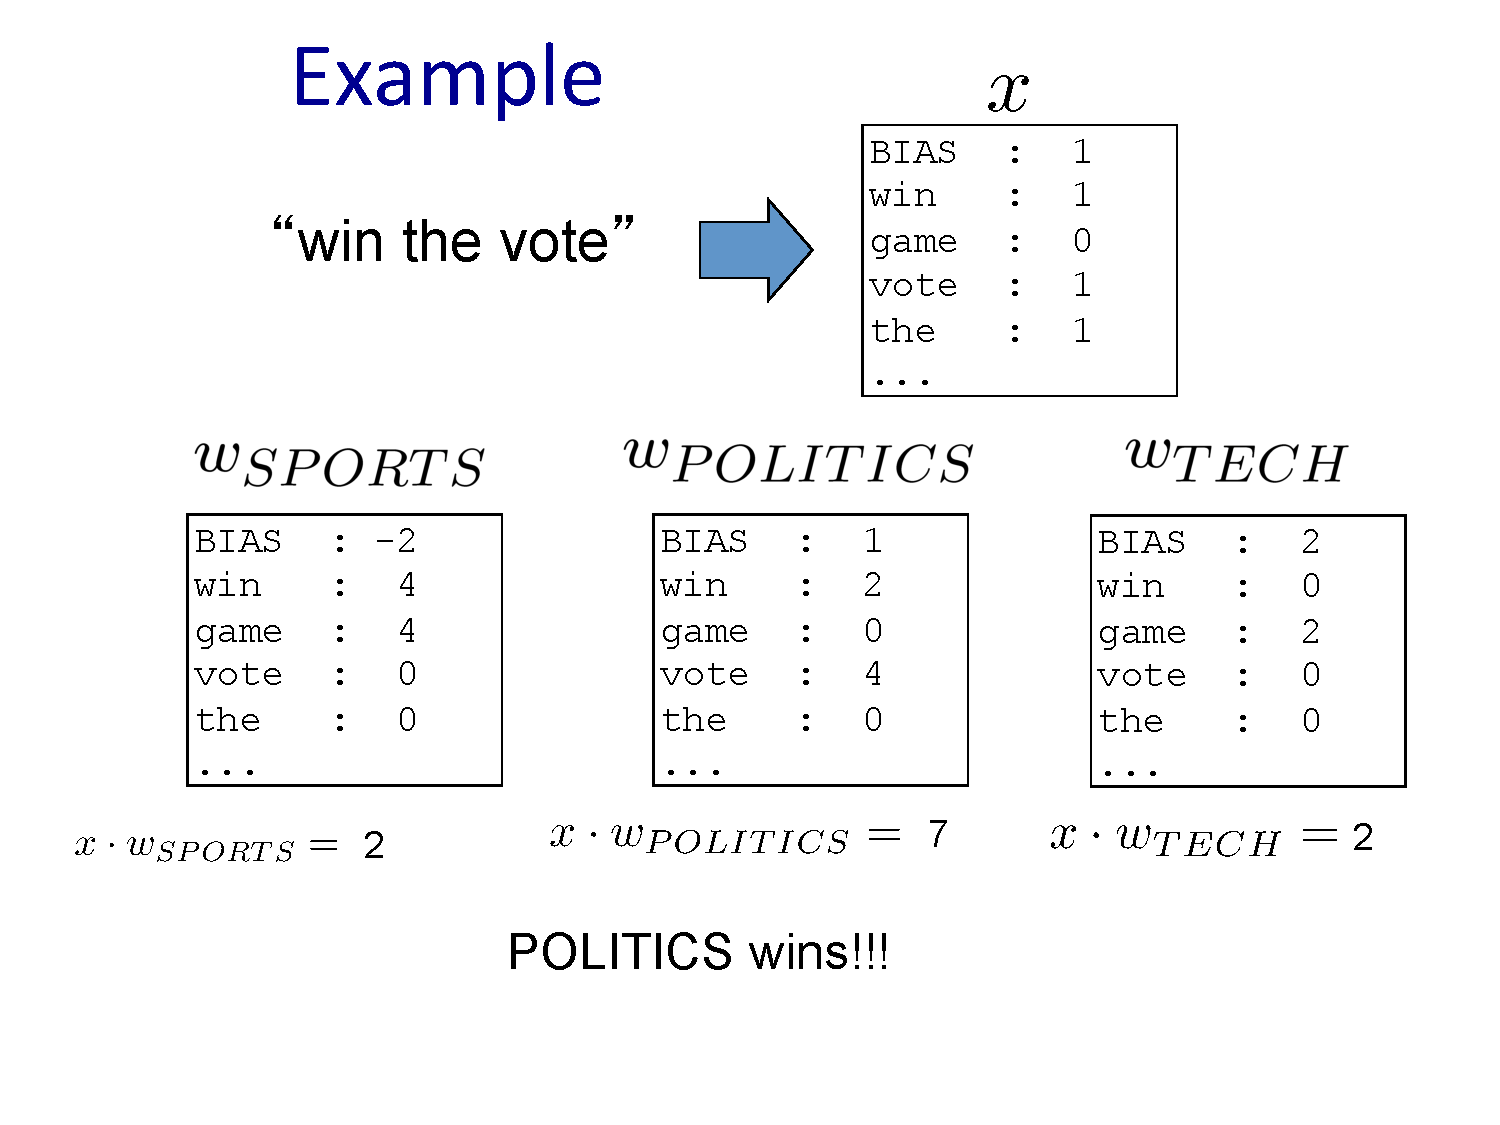
\includegraphics[width=2.5in]{figures/perceptron_multiclass--win_the_vote.pdf}

 \subsubsection{Binary Perceptron Algorithm}
 \begin{itemize}
 	\item start with zero weights: $w_y=0$
	\item for $ t = 1 \dots T$ (T passes over the data):
		\begin{itemize}
			\item for $i = 1 \dots n$ (each training example)
			\begin{itemize}
				\item  Classify with current weights: \hfill \\
					(no more $ y = sign(w_y \cdot x^i)$) \hfill \\
					instead:  $y= \argmax_y w_y \cdot x^i$ \hfill \\
				\item if correct (i.e. $y = y^i$), don't change weights.
				\item if it was wrong, update two vectors: \hfill \\
					$w_y = w_y -x^i$ \hfill \\
					$w_{y^i} = w_{y^i} -x^i$ \hfill \\
					??? Add or subtract from the one that gave you the argmax? ???
			\end{itemize}
		\end{itemize}
 \end{itemize}
 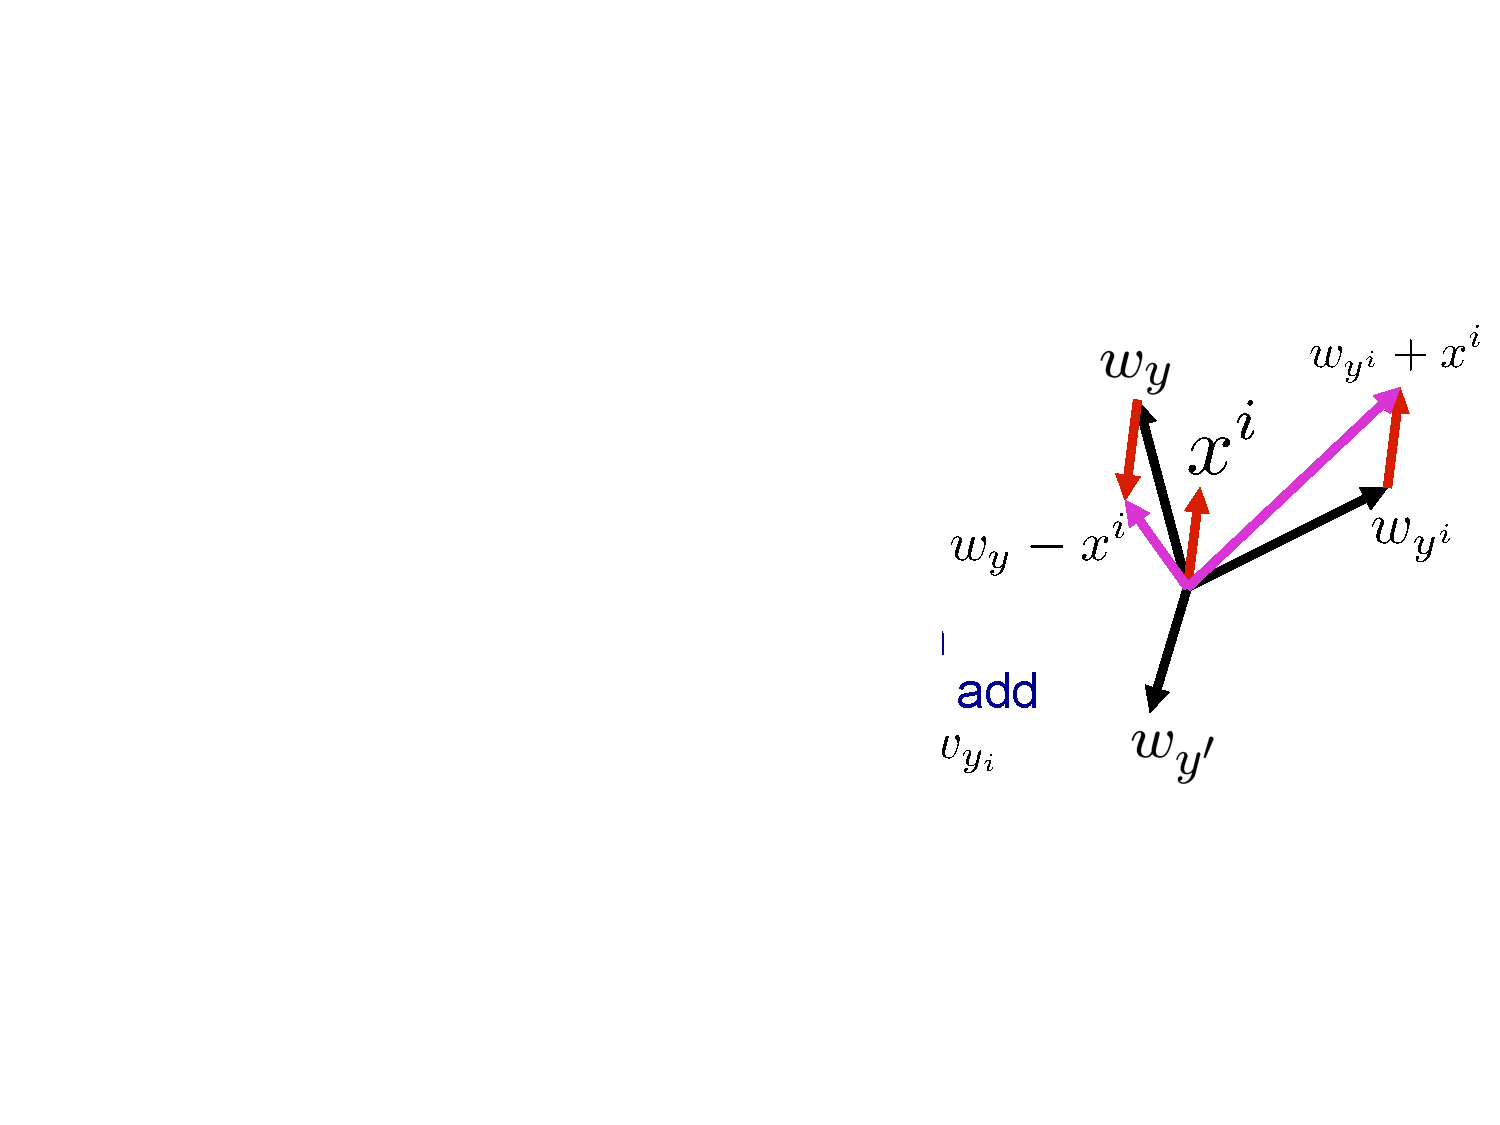
\includegraphics[width=1.0in]{figures/multi_perceptron_rule.pdf}
 
 \subsection{Linear Separability}
 \subsubsection{binary case}
Recall $ \displaystyle  ||x||_2 = \sqrt{\sum_i x_i^2}$ 
 
 The data is linearly separable with margin $\gamma$ if:   \hfill \\
$\exists .w \forall t . y^t (w \cdot x^t) \geq \gamma > 0$.  \hfill \\
Plain english: the data is linearly separable if there exists a w that has a margin greater than zero for all points $t$.  \hfill \\
Note: for $y^t = 1$, $w \cdot x^t \geq \gamma$ and for $y^t = -1$, $w \cdot x^t \leq -\gamma$.  \hfill \\
Plain english: points having label = 1 have a dot product that is greater than $\gamma$, and points that have label = -1 have a dot product that is more negative than $-\gamma$.  \hfill \\
 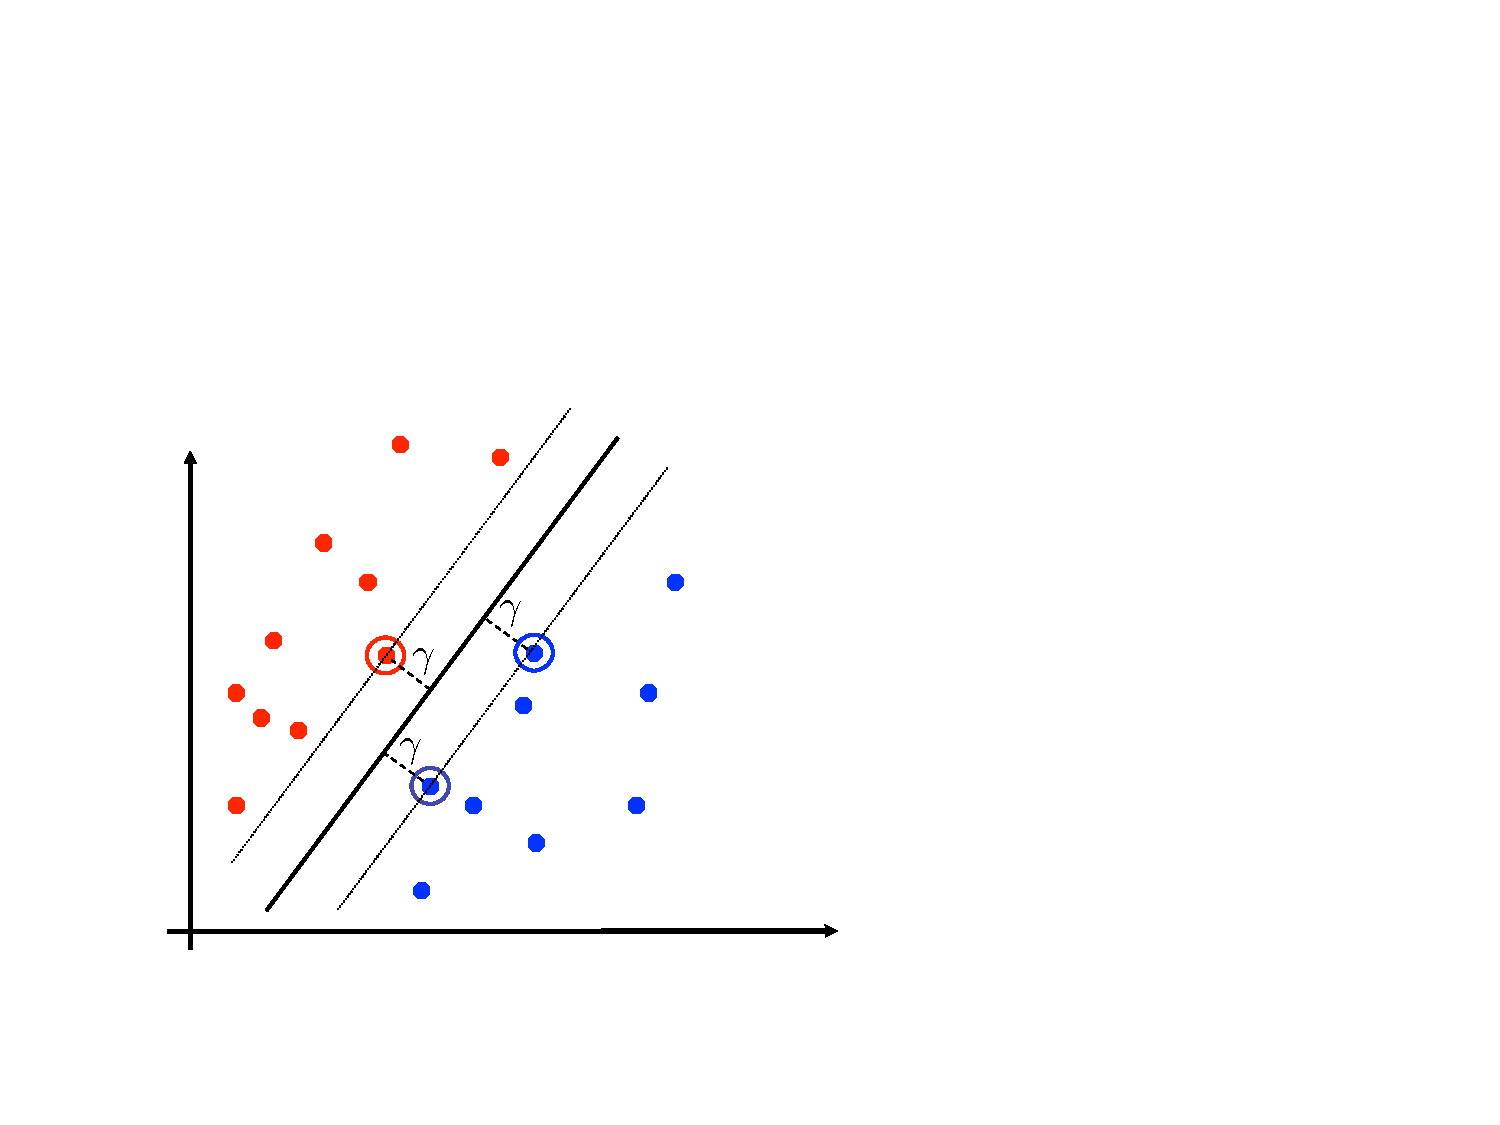
\includegraphics[width=1.0in]{figures/lin_sep_margin.pdf}
 
 \subsubsection{maximum number of mistakes for training linearly separable binary data}
Here, assume the data is separable with margin $\gamma$ and the weight vector is a unit vector: \hfill \\
In math notation, this is: $\exists w^*$ such that $||w^*||_2 = 1$ and $\forall t. y^t(w^* \cdot x^t) \geq \gamma$.) \hfill \\
Recall that you can scale your $w$ (weight) vector(s) by any constant because all you care about is sign($w \cdot x$),
but that this scales your $\gamma$.  You are just multiplying the equation above by a constant.  \hfill \\

Also assume some maximum radius R for your data points:  
$\forall t. ||x^t||_2 \leq R$ \hfill \\
Then the number of mistakes (parameter updates) made by the perceptron is bounded by 
$\displaystyle mistakes \leq \frac{R^2}{\gamma^2}$. \hfill \\
For full inductive proof, see slides.  
Strategy: let $w^k$ be the weights after the k-th update (mistake).  
Then $k^2 \gamma^2 \leq ||w^k||_2^2 \leq k R^2$ \hfill \\
Therefore $k \leq \frac{R^2}{\gamma^2}$.  \hfill \\
\textbf{If there is a linear separator, the Perceptron will find it!}
		
\subsection{Logistic Regression \& Perceptron similarities}
\underline{Logistic regression}:  \hfill \\
In vector notation, y is in the set $\{ 0, 1\}$. \hfill \\
$w = w + \nu \sum_j [y^j - P(y^j | x^j, w))] x^j$ \hfill \\

\underline{Perceptron}:  \hfill \\
When y is in $\{ 0, 1\}$: \hfill \\
$w = w + [y^j - sign^0(w \cdot x^j)] x^j$  \hfill \\
Note: sign$^0(z) =  + 1$ if $z > 0$ and 0 otherwise.  \hfill \\
\hfill \\
Differences:   \hfill \\
1. Online vs. batch learning.  Logistic regression is batch, Perceptron is on-line.  \hfill \\
2. Logistic is probabilistic and Perceptron is error-driven. 
 


